\documentclass{standalone}

\usepackage{tikz}

\begin{document}

%\begin{center}

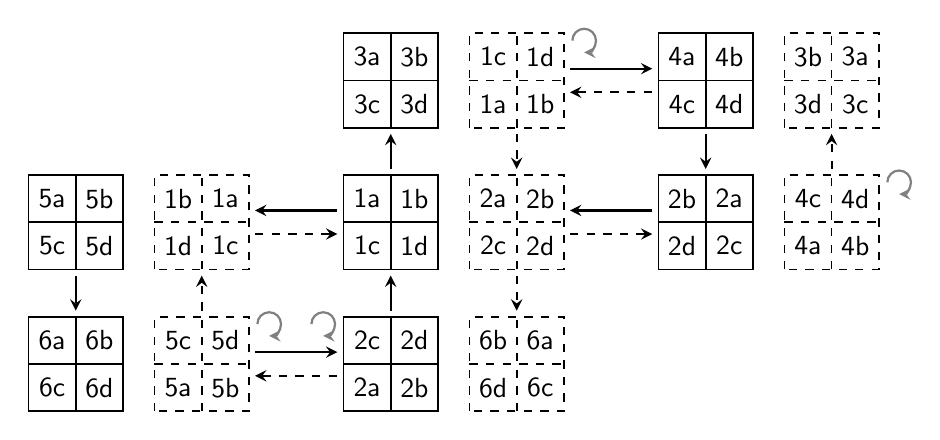
\begin{tikzpicture}[
    >=stealth,
    font=\sffamily,
    % Estilo padronizado para as setas retas: afasta levemente das bordas
    seta/.style={thick, shorten >=2pt, shorten <=2pt}
]

% =========================================================
% === PARÂMETROS DA GRADE LÓGICA (3 Colunas x 3 Linhas) ===
% =========================================================
\def\distCol{4}    % Distância entre os CENTROS das 3 Colunas Principais
\def\distSubCol{1.6} % Distância horizontal entre os 2 quadrados DENTRO da mesma coluna
\def\distLinY{1.8}   % Distância vertical entre as linhas (Top, Mid, Bot)
\def\sepSetas{0.15}  % Separação das setas horizontais duplas (em cm)
% =========================================================

% Macro para desenhar cada matriz 2x2
% #1: Nome do node (para conectar as setas)
% #2, #3: Coordenadas X e Y do centro
% #4: Estilo da borda (solid ou dashed)
% #5, #6, #7, #8: Conteúdo das células
\def\matrixbox#1(#2,#3)[#4]#5#6#7#8{
    % O uso de chaves duplas ({#2}) garante que a matemática seja calculada pelo TikZ
    \node[minimum size=1.2cm, inner sep=0pt] (#1) at ({#2},{#3}) {};
    \begin{scope}[shift={({#2},{#3})}]
        \draw[#4, semithick] (-0.6,-0.6) rectangle (0.6,0.6);
        \draw[#4, semithick] (0,-0.6) -- (0,0.6);
        \draw[#4, semithick] (-0.6,0) -- (0.6,0);
        \node at (-0.3, 0.3) {#5};
        \node at ( 0.3, 0.3) {#6};
        \node at (-0.3,-0.3) {#7};
        \node at ( 0.3,-0.3) {#8};
    \end{scope}
}

% --- Definição das matrizes (Nodes) utilizando o sistema de Grade ---

% --- COLUNA 1 (Esquerda) : Centro em X = -\distCol ---
% Linha Mid (Y = 0)
\matrixbox{L2}({-\distCol - \distSubCol/2}, 0)[solid]{5a}{5b}{5c}{5d}
\matrixbox{L1}({-\distCol + \distSubCol/2}, 0)[dashed]{1b}{1a}{1d}{1c}
% Linha Bot (Y = -\distLinY)
\matrixbox{DL2}({-\distCol - \distSubCol/2}, -\distLinY)[solid]{6a}{6b}{6c}{6d}
\matrixbox{DL1}({-\distCol + \distSubCol/2}, -\distLinY)[dashed]{5c}{5d}{5a}{5b}


% --- COLUNA 2 (Central) : Centro em X = 0 ---
% Linha Top (Y = \distLinY)
\matrixbox{U}({-\distSubCol/2}, \distLinY)[solid]{3a}{3b}{3c}{3d}
\matrixbox{R1}({\distSubCol/2}, \distLinY)[dashed]{1c}{1d}{1a}{1b}
% Linha Mid (Y = 0)
\matrixbox{C}({-\distSubCol/2}, 0)[solid]{1a}{1b}{1c}{1d}
\matrixbox{DR1}({\distSubCol/2}, 0)[dashed]{2a}{2b}{2c}{2d}
% Linha Bot (Y = -\distLinY)
\matrixbox{D}({-\distSubCol/2}, -\distLinY)[solid]{2c}{2d}{2a}{2b}
\matrixbox{DDR1}({\distSubCol/2}, -\distLinY)[dashed]{6b}{6a}{6d}{6c}


% --- COLUNA 3 (Direita) : Centro em X = \distCol ---
% Linha Top (Y = \distLinY)
\matrixbox{R2}({\distCol - \distSubCol/2}, \distLinY)[solid]{4a}{4b}{4c}{4d}
\matrixbox{R3}({\distCol + \distSubCol/2}, \distLinY)[dashed]{3b}{3a}{3d}{3c}
% Linha Mid (Y = 0)
\matrixbox{DR2}({\distCol - \distSubCol/2}, 0)[solid]{2b}{2a}{2d}{2c}
\matrixbox{DDR3}({\distCol + \distSubCol/2}, 0)[dashed]{4c}{4d}{4a}{4b}


% --- Setas Verticais (Se auto-ajustam com a variação de \distLinY) ---
\draw[->, seta] (L2.south) -- (DL2.north);
\draw[->, dashed, seta] (DL1.north) -- (L1.south);
\draw[->, seta] (D.north) -- (C.south);
\draw[->, seta] (C.north) -- (U.south);
\draw[->, dashed, seta] (R1.south) -- (DR1.north);
\draw[->, dashed, seta] (DR1.south) -- (DDR1.north);
\draw[->, seta] (R2.south) -- (DR2.north);
\draw[->, dashed, seta] (DDR3.north) -- (R3.south);


% --- Setas Horizontais (Cruzam a área vazia entre as grandes colunas) ---
% Entre Coluna 1 (L1) e Coluna 2 (C)
\draw[<-, seta] ([yshift=\sepSetas cm]L1.east) -- ([yshift=\sepSetas cm]C.west);
\draw[->, dashed, seta] ([yshift=-\sepSetas cm]L1.east) -- ([yshift=-\sepSetas cm]C.west);

% Entre Coluna 1 (DL1) e Coluna 2 (D)
\draw[->, seta] ([yshift=\sepSetas cm]DL1.east) -- ([yshift=\sepSetas cm]D.west);
\draw[<-, dashed, seta] ([yshift=-\sepSetas cm]DL1.east) -- ([yshift=-\sepSetas cm]D.west);

% Entre Coluna 2 (R1) e Coluna 3 (R2)
\draw[->, seta] ([yshift=\sepSetas cm]R1.east) -- ([yshift=\sepSetas cm]R2.west);
\draw[<-, dashed, seta] ([yshift=-\sepSetas cm]R1.east) -- ([yshift=-\sepSetas cm]R2.west);

% Entre Coluna 2 (DR1) e Coluna 3 (DR2)
\draw[<-, seta] ([yshift=\sepSetas cm]DR1.east) -- ([yshift=\sepSetas cm]DR2.west);
\draw[->, dashed, seta] ([yshift=-\sepSetas cm]DR1.east) -- ([yshift=-\sepSetas cm]DR2.west);


% --- Setas Circulares (Cinza, atreladas aos blocos) ---
\draw[->, gray, thick] ([xshift=0.1cm,yshift=-0.1cm]DL1.north east) arc (180:-90:0.15cm);
\draw[->, gray, thick] ([xshift=-0.4cm,yshift=-0.1cm]D.north west) arc (180:-90:0.15cm);
\draw[->, gray, thick] ([xshift=0.1cm,yshift=-0.1cm]R1.north east) arc (180:-90:0.15cm);
\draw[->, gray, thick] ([xshift=0.1cm,yshift=-0.1cm]DDR3.north east) arc (180:-90:0.15cm);

\end{tikzpicture}
%\end{center}

\end{document}
